\chapter{RESULTS AND DISCUSSION}
The outputs of the program are compared against the output of the software MDLHydroD. The devlopment of the 
MDLHydroD software is explained in \cite{guha2013development} and \cite{guha2015estimation}.
For comparison KCS and KVLCC2 vessels are considered. 

\section{KCS Vessel}
Input parameters for KCS are given in the following table.
\begin{table}[H]
    \centering
    \begin{tabular}{|c|c|}
        \hline
        parameter & value \\ 
        \hline
        \title{something}
        something & something \\
        something & something \\
        \hline
    \end{tabular}
    \caption{Parameters KCS vessel}
    \label{tab:kcs_inp}
\end{table}

\subsection{Added Mass}
\begin{figure}
    \centering
    \begin{subfigure}[b]{0.45\textwidth}
        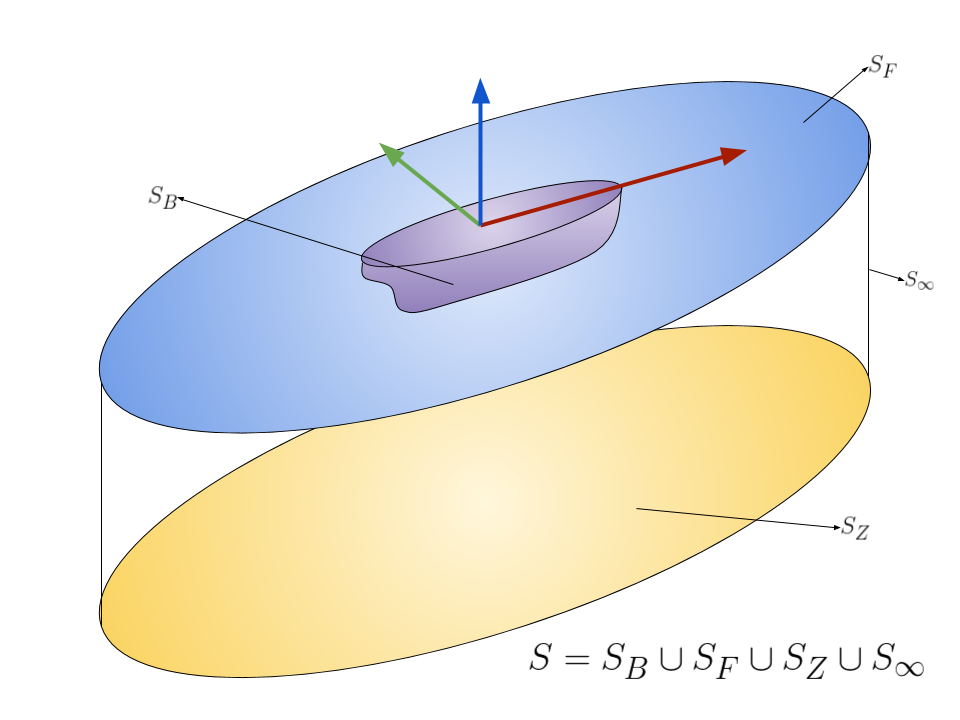
\includegraphics[width=\textwidth]{photos/boundary_surfaces.png}
        \caption{$A_{11}$}
    \end{subfigure}
    \begin{subfigure}[b]{0.45\textwidth}
        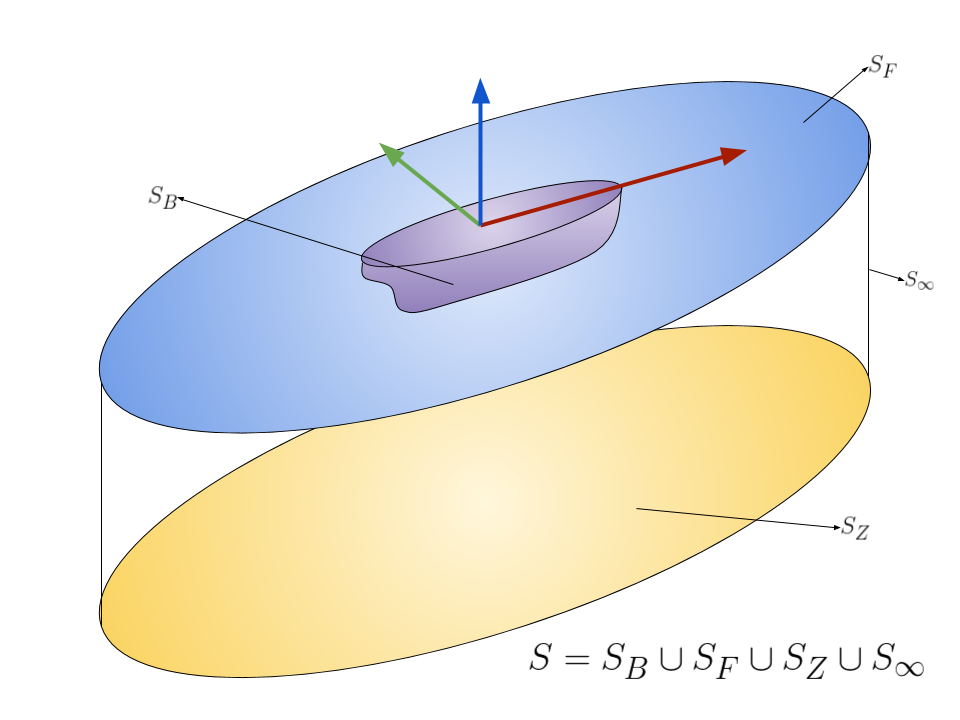
\includegraphics[width=\textwidth]{photos/boundary_surfaces.png}
        \caption{$A_{22}$}
    \end{subfigure}
    \caption{KCS vessel added mass comparison}
    \label{fig:kcs_addedmass}
\end{figure}
\subsection{Radiation Damping}
\subsection{Froude Krylov Force}
\subsection{Scattering Force}

\section{KVLCC Vessel}
Input parameters for KVLCC2 are given in the following table.
\begin{table}[H]
    \centering
    \begin{tabular}{|c|c|}
        \hline
        parameter & value \\ 
        \hline
        \title{something}
        something & something \\
        something & something \\
        \hline
    \end{tabular}
    \caption{Parameters KCS vessel}
    \label{tab:kvlcc2_inp}
\end{table}